\errorstopmode

\documentclass[10pt]{article} % Font size - 10pt, 11pt or 12pt

\usepackage[hmargin=1.25cm, vmargin=1.5cm]{geometry} % Document margins

\usepackage[usenames,dvipsnames]{xcolor} % Allows the definition of hex colors

% Fonts and tweaks for XeLaTeX
\usepackage{fontspec,xltxtra,xunicode}
\defaultfontfeatures{Mapping=tex-text}
%\setmonofont[Scale=MatchLowercase]{Andale Mono}

% Colors for links, text and headings
\usepackage{hyperref}
\definecolor{linkcolor}{HTML}{506266} % Blue-gray color for links
\definecolor{shade}{HTML}{F5DD9D} % Peach color for the contact information box
\definecolor{text1}{HTML}{2b2b2b} % Main document font color, off-black
\definecolor{headings}{HTML}{701112} % Dark red color for headings
% Other color palettes: shade=B9D7D9 and linkcolor=A40000; shade=D4D7FE and linkcolor=FF0080

\hypersetup{colorlinks,breaklinks, urlcolor=linkcolor, linkcolor=linkcolor} % Set up links and colors

\usepackage{fancyhdr}
\usepackage{amsmath}
\usepackage{amssymb}
\usepackage{verbatim}
\pagestyle{fancy}
\fancyhf{}

\renewcommand{\headrulewidth}{0pt} % Get rid of the default rule in the header

\usepackage{titlesec} % Allows creating custom \section's

% Format of the section titles
\titleformat{\section}{\color{headings}
\scshape\Large\raggedright}{}{0em}{}[\color{black}\titlerule]

\title{Dynein notes}
\author{Elliott Capek}
\titlespacing{\section}{0pt}{0pt}{5pt} % Spacing around titles

\begin{document}

\maketitle{}

\subsection{Calculating one/bothbound times of experimental dynein}
In order to fit parameters, a goodness metric for a simulation is needed. Time spent in onebound and bothbound states are good metrics. These values are calculated here.\\

\newcommand\tbb{\left<t_{bb}\right>}
\newcommand\tob{\left<t_{ob}\right>}
\newcommand\tstep{\left<t_{step}\right>}
\newcommand\tproc{\left<t_{processivity}\right>}
\newcommand\kub{k_{ub}}
\newcommand\kb{k_{b}}
\newcommand\ko{k_{dis}}

\begin{itemize}
\item $\tbb$: Time in bothbound per step
\item $\tob$: Time in onebound per step
\item $\tstep$: Time of a single step. $\tstep=\tbb+\tob$.
\item $P_{bb}$: Probability of being bothbound per unit time. $P_{bb} = \frac{\tbb}{\tstep}$
\item $P_{ob}$: Probability of being onebound per unit time. $P_{ob} = \frac{\tob}{\tstep}$
\item $\kub$: Rate of unbinding per unit time while in bothbound. $\kub = \tbb^{-1}$
\item $\kb$: Rate of binding per unit time while in onebound. $\kb = \tob^{-1}$
\item $\ko$: Rate of unbinding per unit time while in onebound. $\ko = P_{ob}\kub$
\item $\tproc$: Time bound to microtubule before dissociation. step length / velocity $= \ko^{-1}$
\end{itemize}

$\tbb$ and $\tob$ can thus be defined in terms of observables $\tstep$ and $\tproc$:

\begin{align*}
  \ko &= P_{ob}\kub = \frac{\tob}{\tstep\tbb}\\
  &= \frac{\tstep-\tbb}{\tstep\tbb}\\
  &= \frac{\tstep-\tbb}{\tstep\tbb}\\
  \tproc &= \frac{\tstep\tbb}{\tstep-\tbb}\\
  \tbb &= \frac{\tproc\tstep}{\tproc+\tstep}\\
  \tob &= \tstep-\tbb\\
  &= \tstep - \frac{\tstep\tproc}{\tstep+\tproc}\\
  &= \frac{\tstep^2}{\tstep+\tproc}\\
  \frac\tob\tbb &= \frac{\tstep}{\tproc}
\end{align*}

Thus, by the above equations and data from various sources, estimates on $\tbb$ and $\tob$ can be made.\\

\begin{figure}[h]
  \centering
  \begin{tabular}{| c | c | c | c | c | c | c |}
    \hline
    Source & Velocity & $\left<L_{step}\right>$ & $\tstep$ & $\tproc$ & $\tbb$ & $\tob$ \\ \hline
    Weihong 2012 GST-dimerized & 134nm/s & 8nm & 0.06s & 7.9s & 0.0595s & 4.52e-4\\ \hline
    Higuchi 2006 & 800nm/s &  &  &   &   & \\ \hline
    Schroer 2000 native 2mM ATP w/ 210nm beads            & 700nm/s &  & 0.011s & 1s    & 0.011s & 1.3e-4\\ \hline
    Schroer 2000 native 2mM ATP w/ 210nm beads + dynactin & 700nm/s &  & 0.011s & 2.14s & 0.011s & 6e-5\\ \hline
    Vale    2006 GST-dimerized 1mM + qdots                & 87 nm/s &  & 0.09s  & 13.8s & &\\ \hline
    Schroer 2000 organic dye-labelled full-length dynein & 120nm/s &  &  &  &  & \\ \hline
    
  \end{tabular}
  \caption{Experimental values for fitting.}{Table calculating estimates for $\tbb$ and $\tob$.}
  \label{table:time-parameter-table}
\end{figure}

\section{Physical Parameters}

\begin{figure}
  \centering
  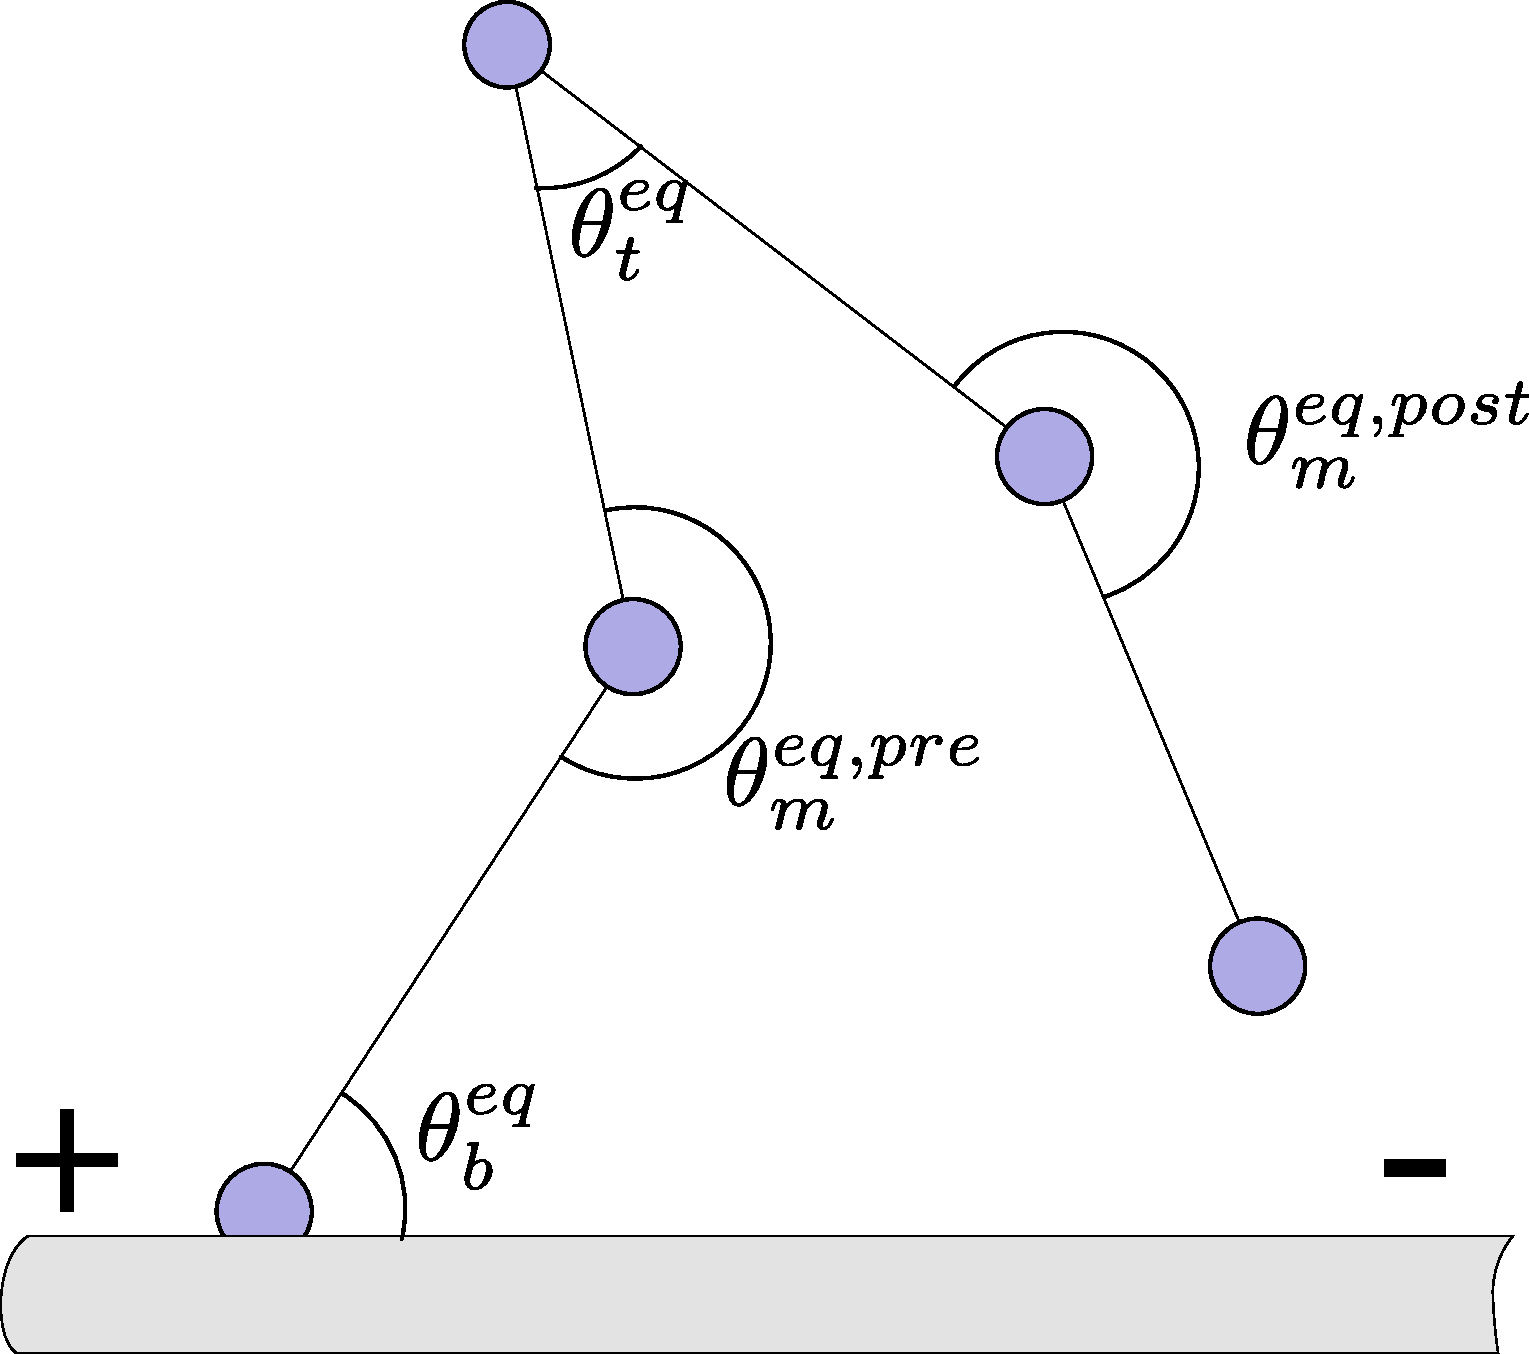
\includegraphics[width=.45\textwidth]{figures/equilibrium-onebound}
  \caption{Definition of equilibrium angles.}
  \label{fig:eq_angles}
\end{figure}

%% \begin{center}
%%   \begin{tabular}{| l | l | l | l | l | l | l | l | l |}
%%     \hline
%%     & Winch (Sarlah) & Schmidt & Lin & PyMol 3VKH & PyMol 4RH7 & Redwine & Kon & Burgess \\\hline
%%     $L_s$ & 12nm & & & 21.0nm & 22.1nm & & & \\ \hline
%%     $L_t$ &  7nm & & & & 11.15nm & & & \\ \hline
%%     $R_b$ &  & & & 1.57nm & 1.45nm & & & \\ \hline
%%     $R_m$ &  7nm & & & 7.36nm & 6.3nm & & & \\ \hline
%%     $R_t$ &  & & & & 2.16nm & & & \\ \hline
%%     $\theta_{m}^{Pre}$ & 250$^{\circ}$ & & 171$^{\circ}$ & & & & & 160\\ \hline
%%     $\theta_{m}^{Post}$ & 330$^{\circ}$ & & 137.5$^{\circ}$ & & & & & 136\\ \hline
%%     $\theta_{b}$ & 56$^{\circ}$ & & 63.5$^{\circ}$ & & & & & \\ \hline
%%     $\theta_{t}$ & 0$^{\circ}$ & & & & & & & \\ \hline
%%     $k_{ub}$ & $180 s^{-1,a}$ & & & & & & $90.2 \pm 4.5$& \\ \hline
%%     $k_b$ & $5000 s^{-1,b}$ & & & & & & & \\ \hline
%%     $\Delta G_{bind, bb}$ & & & & & & -71 kJ/mol & & \\ \hline
%%     $\Delta G_{bind, ob}$ & & & & & & -37 kJ/mol & & \\ \hline
%%     $c_t$ & & & & & & & & \\ \hline
%%     $c_m$ & & & & & & & & \\ \hline
%%     $c_b$ & & & & & & 140 kJ/mol & & \\ \hline
%%   \end{tabular}
%% \end{center}

\textbf{Table moved to real elliott thesis!}

---- not sure if the Lin angles are right, since measuring the angle that the tail makes is \textit{not} necessarily the angle the angle the linker makes ----\\

a: Sarlah \textit{et al} gives us two different rate constants which could represent the bothbound to onebound transition: motor dissociation from the microtubule ($k_{-MT} = 460 s^{-1}$) and ATP hydrolysis/taking on the prestroke conformation ($k_{RS} = 180 s^{-1}$). We take the rate-limiting step $k_{RS}$ as our transition rate from bothbound to onebound since it is the slower of the two.\\

b: There are several Sarlah \textit{et al} rate constants we could use for the onebound to bothbound rate constant: binding to the microtubule ($k_{+MT} = 10^4 s^{-1}$), releasing a phosphate from hydrolysis ($k_{-Pi} = 5000 s^{-1}$) or the power stroke itself ($k_{PS} = 5000 s^{-1}$). We choose to represent the transition with $k_{-Pi} = 5000 s^{-1}$ because all these rates are fairly similar. We do not want to use the MT-binding rate because it could include both binding kinetics as well as MT-search kinetics, the latter of which we do not want to include in our binding rate.\\

\subsection{Stalk and tail length}
Sarlah et. al use stalk and tail lengths of 12 and 14 nm, respectively. We used PyMol to examine the crystal structures 3VKH and 4RH7 (pre and post-powerstroke) to find these values. The linker is roughly residues 1250-1510, calculated by eye.\\

\subsection{Finding Arrhenius preexpontential from k}
Papers often supply rate constants for various transitions. Our model uses Arhennius-type rates which take into account the change in conformational energy from switching equilibrium angles, so we must convert between free energy and rates:

\begin{align*}
  k_{bind} &= Ae^{-\beta(\Delta G_{bind} + \Delta G_{conf})}\\
  k_{bind} &= \left(Ae^{-\beta\Delta G_{bind}}\right)e^{-\beta\Delta G_{conf}}\\
  k_{bind} &= Be^{-\beta\Delta G_{conf})}\hspace{2cm}\mbox{B constant at constant T}\\
  \left<k_{bind}\right> &= \left<Be^{-\beta\Delta G_{conf}}\right>\\
  \left<k_{bind}\right> &= Be^{-\beta\Delta \left<G_{conf}\right>}\\
  \left<\Delta G_{conf}\right> &= \frac{1}{2}k_BT = \frac12\beta^{-1}\hspace{2cm}\mbox{David, what was the justification for this again?}\\
  \left<k_{bind}\right> &= Be^{-1/2}\\
  \rightarrow B &= k_{bind}\sqrt{e}
\end{align*}

\subsection{Properly implementing binding rates}
To determine if it is time to do a state transition, we calculate the per-timestep
transition probability $k_b/dt$, pick a number between zero and one, and transition
if our number was the lower of the two.\\

One issue with this is the rate constant $k_b$ is calculated experimentally from an
ensemble of dynein, and doesn't take into account how transitions are much more likely in some orientations than others. In reality, dynein will only bind to the MT when
its binding domain is less than 0.2nm away from a binding site.\\

To fix this, we define a parameter $n$, the time fraction onebound dynein is capable
of binding. Then a weighted average of the bindable and non-bindable rate constants
looks like:

\begin{equation*}
  nk_{bindable} + (n-1)k_{nonbindable} = k_b
\end{equation*}

Since we say $k_{nonbindable} = 0$, $k_{bindable}$, our effective rate constant of
binding, is $k_b/n$. Thus our preexponential Arrenhius factor is (see above):

\begin{equation*}
  B = \frac{k_{b}\sqrt{e}}{n}
\end{equation*}

\subsubsection{Calculating $n$}
A script, \verb|simulations/get_binding_time_fraction.py|, calculates how often
a onebound dynein spends in a bindable state:

\verbatiminput{../simulations/simulation_results/binding_time_fraction.txt}

\subsection{Calculating $\Delta G_{bind}$}
Based on Van der Spoel \textit{et. al.}, $\Delta H_{HB} = 10.6kJ/mol$ for water molecules forming a single hydrogen bond. Based on another paper (Anderson \textit{et al}), the
``stabilizing energy'' of a single salt bridge (H-bond between charged molecules) is about 16 kJ/mol.\\

Based on the interpreted bonds from crystal structures of the MTBD-MT complex shown in Redwine \textit{et. al}, there are 5.9 salt bridges in the high-affinity MTBD-MT
complex and 3.1 in the low-affinity complex. Thus if we guess the free energy of a salt bridge as 12 kJ/mol, we can estimate binding energies as:

\begin{align*}
  \Delta G_{bind, high-affinity} &= -71 \mbox{ kJ/mol}\\
  \Delta G_{bind, low-affinity} &= -37 \mbox{ kJ/mol}\\
\end{align*}

\subsection{Estimating $c_b$ spring constant}
If the energy of binding of the MTBD foot to the MT is -71 kJ/mol, we can get a rough estimate of the spring constant for the binding domain. We say that
$\Delta \theta \approx 0$ corresponds to being fully bound and $\Delta \theta \approx 1$ corresponds to breaking all salt bridges and being unbound. Thus:

\begin{align*}
  \frac 12 c_b \Delta \theta_{ba}^2 = \Delta G_{bind, high} &\rightarrow c_b = 2\Delta G_{bind, high} \approx 140 \mbox{ kJ/mol}\\
\end{align*}

\subsection{ATP Concentration from Weihong's Paper}
Weihong says in the Supplemental Methods section that the ATP concentration of the ``dynein motility buffer'' used to take his videos was 1mM, with no added ADP or Pi.\\

\subsection{Parameter hunt}
Lots of different manual simulations and their outcomes.

\begin{center}
  \begin{tabular}{| l | l | l | l | l | l | l | p{3cm} | p{2cm} | p{5cm} |}
    \hline
    Ls & Lt & kb & kub & cm & cb & ct & $\Big<P(\mbox{unbind per dt})\Big>$ & $\Big<\mbox{step time}\Big>$ & errors\\\hline
    22.1 & 11.1 & 5000 & 5000 & 0.02 & 0.02 & 0.02 & NA      & NA     & keeled over after ns\\\hline
    22.1 & 11.1 & 5000 & 5000 & 0.11 & 0.11 & 0.11 & $9e-9 $ & 1.7e-4 & keeled over after ns\\\hline
    22.1 & 11.1 & 5000 & 5000 & 0.18 & 0.18 & 0.18 & $4e-9 $ & 3.4e-4 & no error yet\\\hline
    22.1 & 11.1 & 5000 & 5000 & 0.23 & 0.23 & 0.23 & $3e-9 $ & 2.9e-4 & no error yet\\\hline
    22.1 & 11.1 & 5000 & 5000 & 0.58 & 0.58 & 0.58 & $2e-10$ & 3.3e-4 & no error yet\\\hline
    22.1 & 11.1 & 5000 & 3500 & 1.00 & 1.00 & 1.00 & ?? & 6.8e-4 & no error yet\\\hline
    22.1 & 11.1 & 5000 & 2000 & 1.00 & 1.00 & 1.00 & ?? & 1.6e-3 & weirdly stepped so L is around zero (0.04), maybe write a nudge to prevent this?\\\hline
    22.1 & 11.1 & 5000 & 1000 & 1.00 & 1.00 & 1.00 & ?? & 1.9e-3 & weirdly stepped so L is around zero (0.04), maybe write a nudge to prevent this?\\\hline
    22.1 & 11.1 & 5000 &  100 & 1.00 & 1.00 & 1.00 & ?? & 7.9e-3 & no error yet\\\hline
    22.1 & 11.1 & 5000 & 5000 & 1.16 & 1.16 & 1.16 & $6e-12$ & 8.4e-4 & no error yet\\\hline
    22.1 & 11.1 & 5000 & 5000 & 1.74 & 1.74 & 1.74 & $1e-13$ & 3.3e-3 & no error yet\\\hline
    22.1 & 11.1 & 5000 & 5000 & 2.32 & 2.32 & 2.32 & $7e-16$ & 9.0e-3 & no error yet\\\hline
    22.1 & 11.1 & 5000 & 3500 & 2.32 & 2.32 & 2.32 & ?? & 1.3e-2 & no error yet\\\hline
    22.1 & 11.1 & 5000 & 2000 & 2.32 & 2.32 & 2.32 & ?? & 1.3e-2 & no error yet\\\hline
    22.1 & 11.1 & 5000 & 1000 & 2.32 & 2.32 & 2.32 & ?? & 4.6e-2 & no error yet\\\hline
    22.1 & 11.1 & 5000 &  100 & 2.32 & 2.32 & 2.32 & ?? & ?? & no error yet\\\hline
    22.1 & 11.1 & 5000 & 5000 & 2.90 & 2.90 & 2.90 & $2e-18$ & 7.2e-2 & no error yet\\\hline
    22.1 & 11.1 & 5000 & 5000 & 3.49 & 3.49 & 3.49 & $5e-21$ & ?? & no error yet\\\hline
  \end{tabular}
  \textbf{Old probably wrong angle scheme run data}
\end{center}

\begin{center}
  \begin{tabular}{| l | l | l | l | l | l | l | p{3cm} | p{2cm} | l | p{5cm} |}
    \hline
    Ls & Lt & kb & kub & cm & cb & ct & $\Big<P(\mbox{unbind per dt})\Big>$ & $\Big<\mbox{step time}\Big>$ & run & errors\\\hline
    22.1 & 11.1 & 5000 & 5000 & 0.02 & 0.02 & 0.02 & & & & NaN! tail crashes into MT \\\hline
    22.1 & 11.1 & 5000 & 5000 & 0.11 & 0.11 & 0.11 & & & & NaN! motor crashes into MT \\\hline
    22.1 & 11.1 & 5000 & 5000 & 0.18 & 0.18 & 0.18 & & & & NaN! tail crashes into MT \\\hline
    22.1 & 11.1 & 5000 & 5000 & 0.23 & 0.23 & 0.23 & & $3.7e-4$ & & NaN! tail crashes into MT \\\hline
    22.1 & 11.1 & 5000 & 5000 & 0.58 & 0.58 & 0.58 & & $9.1e-4$ & & NaN! motor crashes into MT \\\hline
    22.1 & 11.1 & 5000 & 5000 & 1.16 & 1.16 & 1.16 & $2.7e-13$ & $6.8e-4$ & & \\\hline
    22.1 & 11.1 & 5000 & 5000 & 1.74 & 1.74 & 1.74 & & & & \\\hline
    22.1 & 11.1 & 5000 & 5000 & 2.32 & 2.32 & 2.32 & & & & \\\hline
    22.1 & 11.1 & 5000 & 5000 & 2.90 & 2.90 & 2.90 & $9.5e-32$ & & & \\\hline
    22.1 & 11.1 & 5000 & 5000 & 3.49 & 3.49 & 3.49 & $2.7e-35$ & & & \\\hline
    22.1 & 11.1 & 5000 & 3500 & 1.00 & 1.00 & 1.00 & $2.7e-12$ & $1.7e-3$ & & NaN! motor crashes into MT\\\hline
    22.1 & 11.1 & 5000 & 3500 & 2.32 & 2.32 & 2.32 & $4.1e-18$ & $5.5e-3$ & & \\\hline
    22.1 & 11.1 & 5000 & 2000 & 1.00 & 1.00 & 1.00 & $1.5e-12$ & $2.2e-4$ & & \\\hline
    22.1 & 11.1 & 5000 & 2000 & 2.32 & 2.32 & 2.32 & $2.2e-18$ & & & \\\hline
    22.1 & 11.1 & 5000 & 1000 & 1.00 & 1.00 & 1.00 & & & & \\\hline
    22.1 & 11.1 & 5000 & 1000 & 2.32 & 2.32 & 2.32 & & & & \\\hline
    %% 22.1 & 11.1 & 5000 &  180 & 1.00 & 1.00 & 1.00 & & $1.8^{-2}$ & & \\\hline
    %% 22.1 & 11.1 & 5000 &  180 & 1.30 & 1.30 & 1.30 & & $1.9^{-2}$ & & \\\hline
    %% 22.1 & 11.1 & 5000 &  180 & 1.60 & 1.60 & 1.60 & & $1.9^{-2}$ & & \\\hline
    %% 22.1 & 11.1 & 5000 &  180 & 1.90 & 1.90 & 1.90 & & $1.9^{-2}$ & & \\\hline
    %% 22.1 & 11.1 & 5000 &  180 & 2.10 & 2.10 & 2.10 & & $1.9^{-2}$ & & \\\hline
    22.1 & 11.1 & 5000 &  180 & 2.25 & 2.25 & 2.25 & & $1.9^{-2}$ & & \\\hline
    %% 22.1 & 11.1 & 5000 &  180 & 2.40 & 2.40 & 2.40 & & $1.9^{-2}$ & & \\\hline
    %% 22.1 & 11.1 & 5000 &  180 & 2.55 & 2.55 & 2.55 & & $1.9^{-2}$ & & \\\hline
    %% 22.1 & 11.1 & 5000 &  180 & 2.70 & 2.70 & 2.70 & & $1.9^{-2}$ & & \\\hline
    %% 22.1 & 11.1 & 5000 &  180 & 3.10 & 3.10 & 3.10 & & $1.9^{-2}$ & & \\\hline
    22.1 & 11.1 & 300 &  180 & 2.40 & 2.40 & 2.40 & & $1.9^{-2}$ & & \\\hline
    22.1 & 11.1 & 100 &  180 & 2.40 & 2.40 & 2.40 & & $1.9^{-2}$ & & \\\hline
  \end{tabular}
  \textbf{New possibly right angle scheme run data}
\end{center}

ARE THESE ANGLES RIGHT??????????????\\

If the mean stepping rate from Weihong's paper is about 1 step / .1 seconds, then at a dt of $1e-11$s would lead to a desired unbinding
probability of $1e-11s/.1s = 1e-10$. The stepping probability was determined by printing out a random subset of unbinding probabilities
for the bothbound case, then averaging.\\

A more reliable step time determiner is $\Big<\mbox{step time}\Big>$, which should be around 0.1. This number can be determined from our step time histograms.\\

\section{Papers}
\subsection{Native dynein cryo-EM structure}
Full structure of dynein.\\

\subsection{HC dimerization}
The structure of the dynactin complex and its interaction with dynein -- stuff about HC dimerization, NOT structure\\

Structure of dynactin-dynein. Paper says that ct is pretty loose; loose enough that the angle can rotate 180 to take on the in-vivo state (originally the two motors are 180 degrees apart, but rotate to be parallel). It seems that there is only one dimerization domain at the very N-term of the heavy chain (1-178).\\

Paper says that dynactin may work by separating the two HCs, allowing them to take on an active, bipedal legs-unlocked conformation. Perhaps without this, the two HC legs wrap around each other, or somethign.\\

\subsection{Paper on our model stepping in the proper direction given our angle scheme}
Figure 7 of 'Three-dimensional structure of cytoplasmic dynein bound to microtubules' shows a cartoon interpretation of a dynein-MT crystal structure indicating that a model which has its tail-load towards the + end will step towards the - end of the MT.\\

\subsection{Structure of human cytoplasmic dynein-2 primed for its power stroke}
Schmidt, Carter et al\\

Paper on crystallizing dynein-2 (cytoplasmic) with and without ADP-Vanadate to find the pre- and post-powerstroke structures. They find a different foot-head-tail angle than the Burgess paper (possibly because Burgess crystallized axonemal dynein). Burgess found a ~20 degree shift for axonemal, and schmidt found a 90 degree shift in angle on pre-stroking.\\

\subsection{Tension on the Linker Gates the ATP-Dependent Release of Dynein from Microtubules - Yildiz 2014}
Yildiz shows that dynein only requires one functional head, and an MTBD linker, to walk. He claims that this shows dynein relies on high bb/ob time, not from communication. He does say that linker tension increases ATP hydrolysis rate, which isn't really inter-head connection.\\
Takeaway: linker tension inhibits MT release. Stepping happens lots when the active head is low-tension (near its partner), but not when it is far away.\\

Yildiz found that processivity and velocity are inversely related. This means that the MT-bound to unbound ratio is related to how far the motor can walk. Thus, tuning $k_b$ and $k_ub$ may be a way to alter dynein processivity.\\

A ring domain can be substituted with another protein and still walks, so ring-ring interactions aren't necessary for motion, either.\\

This result means that stalk registry changes aren't necessary for MT unbinding.\\

Abolishing linker swing by making weird constructs inhibits stepping when the linked head is mutated, but not when the unlinked head is muated.\\

There's a better stall-force measurement here than in other assays.\\

\subsection{A Simple Theoretical Model Explains Dynein’s Response to Load}
Yi Qin Gao 2006

Two reaction coordinates. First is where it is in the ATP, ADP-Pi, ADP, Apo cycle. Second is domain orientation and MT binding status position.\\

Stalling force increases by 4-fold when [ATP] goes from 0.1 to 1mM, a much more dramatic change than seen in kinesin. (they cite this claim). Dynein's step size also varies a lot with load -- we could easily test if our model behaves this way, as well.\\

ATP binding rate to apo dynein: $7*1-^5/m/s$

This seems like a good paper to finish eventually. It would be something to compare our results to.\\

\subsection{Interesting Crystal Structures}
\textbf{3VKH} 2.8A x-ray resolution full dynein motor, from Kon 2012 (2.8A crystal structure of the dynein motor domain). Probably what we'll use to get some equilibrium angles and lengths, though not sure if crystal structures are identical to in vivo structures. Discusses amino acid chemistry of the powerstroke and long-distance MTBD/ATPase communication.\\
\textbf{3J67/3J68} 34A EM structure of pre/post motor (from Structural Mechanism of dynein power stroke 2014). Shows in-depth changes to motor, but appears to only be the six ATPases and possibly buttress.
\textbf{3J1T/3J1U} 9.7A EM structure of tightly/loosly bound tubulin-MTBD binding from (Structural basis for microtubule binding and release by dynein).\\
\textbf{4RH7} 2.3A x-ray crystal structure of dynein motor/stalk with ADP.Vi (pre-stroke) from (Structure of human cytoplasmic dynein-2 primed for its power stroke). Could be another good place to get angles for pre-stroke, since 3VKH is post-stroke.\\

\subsection{Single-Molecule Analysis of Dynein processivity and Stepping Behavior}
Vale RD\\
2006 paper on single-molecule analysis of step sizes of dynein. Might have in-vivo velocity information.\\

Cool asside: Dynein can be dissociated from microtubules by adding 5mM ATP. This makes sense, since unbinding rate is proportional to ATP concentration.\\

Report a velocity of $85\pm30$ nm/s. Run length of $1.9\pm0.2\mu m$. Measurements done at $1mM ATP$.\\

Required for walking: two motor domains, but not cargo binding or associated chains.\\

Step length assay conducted at $4 \mu M$ ATP, roughly three orders of magnitude less than \textit{in vivo} ATP concentration.\\ 

Head steps are roughly 8nm, but motor movements per step are 0 for nonmoving and 16-18 for moving motor. This means that our average step size should be about 16nm.\\

Dwell time: probably the average time a domain is bound to the MT? IE the total step time? Although perhaps they only measure dwell times when they are especially long, since the average looks to be around 2s, or ten dynein steps.\\

Stepping rate of 0.13 per second per $\mu M$ ATP. Ten steps per second, consistent with velocity.\\

Forward stepping probability: 0.8\\

Propose the original ``alternate shuffling''/''hand-over-hand'' mechanism, where each head moves past the other, and the tail/centroid moves a half of each motor domain's movement.\\

\subsection{ATP concentration papers}
\paragraph{The Contents of Adenine Nucleotides, Phsphagens and some Glycolytic Intermediates in Resting Muscles from Vertebrates and Invertebrates -- 1975}

Found the following:

\begin{center}
  \begin{tabular}{| l | l |}
    \hline
    Organism & ATP\\ \hline
    Locust flight muscle & 5.8mM\\ \hline
    Rosechafer flight muscle & 8.5mM\\ \hline
    Dogfish white muscle & 4.18mM\\ \hline
    Lab rat thigh & 6.23mM\\ \hline
    Lab rat kidney & 1.71mM\\ \hline
  \end{tabular}
\end{center}

\paragraph{Diversity in ATP concentrations in a single bacterial cell population revealed b quantitate single-cell imaging}

Report $1.54\pm1.22$ mM\\

\paragraph{Bionumbers: http://bionumbers.hms.harvard.edu/search.aspx?log=y\&task=searchbytrmorg\&trm=atp+concentration\&org=}

Growing E. coli: 9.6 mM\\
human blood cell: 1.61 mM\\
Maize: 0.5-1.2 mM\\

\subsection{H-bond $\Delta G$ calculation paper}
van der Spoel, D., J. van Maaren, P., Larsson, P., Timneanu, N. ``Thermodynamics of Hydrogen Bonding in Hydrophilic and Hydrophobic Media'' \textit{J. Phys. Chem. B} 2006: 110, 4393-4398.\\

This paper uses classical simulations of water and alcohols to calculate thermodynamic parameters for the transition state and equilibrium state of water-water and water-alcohol
hydrogen bonds. It uses H-bond lifetime and the Eyring rate equation to calculate transition state $\Delta G$ and number of H bond pairs / unbonded pairs to find equilibrium
$\Delta G$. It then uses a Van't Hoff calculation to find enthalpies and entropies. Raman spectroscopy is shown to find a different enthalpy for water-water H-bonds. Findings:

\begin{center}
  \begin{tabular}{| l | l | l | l | l | l |}
    \hline
    & $\Delta G$ & $\Delta H$ & $T\Delta S$ \\\hline
    Simulation & 5.11 kJ/mol & 9.0 kJ/mol & 4.1 kJ/mol\\ \hline
    Experimental & 10.6 kJ/mol & & \\ \hline
  \end{tabular}
\end{center}

where T = 298.15K.\\

Another study (pH-Induced denaturation of proteins: a single salt bridge contributes 3-5 kcal/mol to the free energy of folding of T4 lysozyme by D. Anderson) found that
a single salt bridge contributes about 16 kJ/mol to stabilizing a protein. We can use these numbers as estimates of the binding energy of the motor.\\

\subsection{Helix sliding in the stalk coiled coil of dynein couples ATPase and microtubule binding}
Takahide Kon, Kenji Imamula, Anthony J Roberts, Reiko Ohkura, Peter J Knight, I R Gibbons, Stan A Burgess \& Kazuo Sutoh\\
Discuss how other work has shown that MT affinity is controlled by registry. They do this study in vivo, and show that there is a coupling between ATPase activity and MT binding which is destroyed by locking the coiled coils into registries.

\textbf{Key findings}
\begin{itemize}
\item CC being unlocked is necessary for MT-affinity sensitivity to ATP, showing ATP-state influences MT-affinity
\item high MT affinity causes high ATPase rate, low MT affinity causes low ATPase rate (presumably bc ATP cannot bind)
\end{itemize}

WT: No ATP -> strong binding, ATP: weak binding\\
Locked in a register: ATP insensitivity\\
MT increases ATPase rate 25x\\
MT doesn't increase locked-register ATPase rate\\
(Thus unlocked registers are necessary for ATPase/MT-binding coupling)\\

They then did a FRET study to show that locking a registry \textit{induces} a change in linker conformation, pre/poststroke.\\

They provide the following explanation of dynein mechanochemical cycle:

\begin{itemize}
\item (apo): strong MT-binding, in $\alpha$ conformation
\item (ATP binding): causes a shift towards the $\beta+$ conformation, causing MT dissociation by lowering affinity
\item (before ATP hydrolysis): dynein performs prestroke, \textit{then} hydrolyzes ATP
\item (during Phosphate or ADP release): MTBD rebinds to MT, returns to $\alpha$ registry, increasing the rate of product release, increasing MT affiniy, AND causing the powerstroke
\item (full release): turns back to apo dynein
\end{itemize}

ATPase and MT cycles are interestingly coupled.

\textbf{ATPase cycle}
\begin{itemize}
\item apo $\rightarrow$ ATP: this is somehow influenced by MT state
\item ATP $\rightarrow$ ADP+Pi: This happens after prestroke, somehow coupled to it or no?
\item ADP+Pi $\rightarrow$ ADP: This ejection (or the ADP ejection) is sped up by MTBD rebinding
\item ADP $\rightarrow$ apo: This ejection doesn't do anything structurally, according to Cianfrocco model
\end{itemize}

\subsection{MTBD-Tubulin complex}
Redwine, W.B. \textit{et. al.} ``Structural basis for microtubule binding and release by dynein. '' Science 2012, 337(6101): 1532–1536.

This is a sub-nanometer MTBD-tubulin complex structure which shows how the complex forms. A cryo-EM structure was acquired, atomic-resolution structures for the high-affinity
MTBD and tubulin dimers were superimposed.  Rigid body docking and molecular dynamics was then used to optimize this structure. Another technique was used to figure out how
the low-affinity MTBD would bind, and yet another technique was used to translate between the low and high-affinity MTBDs to make an animation. Also did this with the Kon
vanadium onebound crystal structure and not much changed.\\

The MTBD-tubulin dimers are on the PDB as 3J1T for the high-affinity and 3J1U for the low-affinity structures.\\

After finding the high- and low-affinity structures for the complexes, the authors guess at what salt bridges form in the two states between MT and MTBD. The reported values are shown in the tables below.\\

\begin{table}
  \parbox{.45\linewidth}{
    \centering
    \begin{tabular}{| l | l |}
      \hline
      Residue & Occupancy \\\hline
      R3382-αE417 & 23\% \\\hline
      R3382-αE420 & 79\% \\\hline
      R3382-αG416 & 40\% \\\hline
      K3299-βE431 & 60\% \\\hline
      K3299-βD427 & 53\% \\\hline
      R3342-βE159 & 51\% \\\hline
      N3310-αG410 & 38\% \\\hline
      L3385-αE415 & 48\% \\\hline
      S3384-αG415 & 27\% \\\hline
      A3383-αE415 & 49\% \\\hline
      R3306-βE196 & 86\%*\\\hline
      R3337-βD199 & 2\%* \\\hline
      R3342-βN197 & 36\%*\\\hline
    \end{tabular}
    \caption{High-affinity MTBD-MT complex salt bridges. RH column is bonds between MTBD and MT, respectively.}
  }
  \hfill
  \parbox{.45\linewidth}{
    \centering
    \begin{tabular}{| l | l |}
      \hline
      Residue & Occupancy \\\hline
      A3383-αE415  & 45\% \\ \hline
      R3382-αG416  & 44\% \\ \hline
      R3382-αE417  & 61\% \\ \hline
      R3382-αE420  & 79\% \\ \hline
      K3299-βE196  & 27\% \\ \hline
      S3307-βR253  & 16\% \\ \hline
      L3385-αE415  & 34\% \\ \hline
      N3310-αK112  & 10\% \\ \hline
    \end{tabular}
    \caption{Low-affinity MTBD-MT complex salt bridges. RH column is bonds between MTBD and MT, respectively.}
  }
\end{table}

From this table we count the number of effective salt bridges in the high/low affinity complexes: 5.9 and 3.1, respectively.\\

Some \textbf{really} cool videos of the MTBD switching from high/low affinity states. If you could get a similar video of the AAA domains binding ATP, these would be really
cool videos to put in a presentation.\\

\subsection{Winch Model (dx.doi.org/10.1016/j.bpj.2014.06.022)}
-Communication between motors and BDs possible through $\alpha$-helix sliding. Bidirectional communication. [24,25]\\
-Pre, post-powerstroke states\\
-Pre-powerstroke: unbound state after ATP hydrolysis (our onebound)\\
-Post-powerstroke: bound state (our bothbound)\\
-Elastic stalk, unlike our rigid one\\
-Only tail angle changes between pre and post-powerstroke\\
-MTBD decides directionality?\\
-Tail-tail interaction, also motor-motor stacking interaction\\
-rate constant simulation, does not do dynamics to take into account time spent in a state\\

\textbf{Physical Parameters from Winch Model paper}:\\
Sarlah et al. use the following physical parameters for Dynein: $L_s = 12$nm binding angle: 34 degrees from vertical, motor
domain radius: 7nm. Their angle scheme is different than ours in that it has the linker/tail facing towards the MT, which looks different
from our facing-up tail. This might be a confusion on our part in the difference between the linker and the tail, but it may not. By assuming the linker starts at the top of the head and points downwards, we can calculate an estimate for tail length as $L_t = 7nm$.

\subsection{Annual Review, 8-state Mechanochemical diagram}
Cianfrocco, M*., DeSantis, M*., Leschziner, A., Reck-Peterson, S. ``Mechanism and Regulation of Cytoplasmic Dynein'' \textit{Annu. Rev. Cell. Dev. Biol.} 2015: 31:83-108.\\

Goes over in detail the various steps of the Dynein chemical cycle. Eight-state model as follows:\\

\begin{enumerate}
\item Dynein begins cycle with AAA1 binding site open.
\item ATP then binds to the AAA1 binding site.
\item ATP binding causes ``ring closure,'' where the AAA1 and AAA2 subdomains shift closer together.
\item Ring closure (ie ATP binding) causes the buttress to shift, causing the MTBD to lose MT affinity.
\item Ring closure (ATP binding) also causes the linker to bend 90 degrees, causing the monomer to enter the pre-powerstroke state. The order of states 4. and 5. is unknown, but entering pre-powerstroke \textit{after} unbinding from the MT causes more directional motion. The role of ATP hydrolysis also is not understood as of this paper (2015).
\item Random walk of the low-MT-affinity MTBD eventually leads to weak rebinding at a new place on the MT.
\item Rebinding causes a change in the MTBD back to its high affinity state. AAA4 moves to prevent steric clash when the linker straightens. AAA5/6 move away from AAA1 and the linker straightens to its post-powerstroke conformation. NOTE: this is distinct from the conformation in steps 1-4 in that AAA1/2 is still closed.
\item The linker shifts some more and AAA1/2 opens up, releasing ADP.
\end{enumerate}

\subsection{Weihong's Dynein stepping data}
Qiu, W., Derr, N., Goodman, B., Villa, E., Wu, D., Shih, W., Reck-Pterson, S. ``Dynein achieves processive motion using both stochastic and coordinated stepping.'' \textit{Nature Structural \& Molecular Biology}. 2012, 19:193-200.\\

Has the stepping histograms we are trying to reproduce computationally.\\

Velocities reported here are probably bad, but the step lengths are good. Step length not influenced by [ATP].\\

At Weihong's 1mM [ATP], the stepping rate for their dynein is $k = 1.78 ± 0.13 s−1$. Thus dynein takes a step roughly every $0.58s$ when in low-ATP conditions. Average velocity at this concentration si $134 ± 60.4 nm s−1$. Run length of $1.06 ± 0.044 µm$.\\

Seems to be a difference between different types of steps: tail steps are a single motion of the tail, and Weihong says are about 10nm (2d). Motions of each motor are 14-16nm. 77\% are forward steps.\\

Head moves half as fast as either motor, suggesting motors move every other step, tail moves each step.\\

It's potentially important to note the dynein species used, though probably not since Weihong didn't mention it much in the paper.\\

\subsection{Pre-powerstroke structure, linker remodel details}
Schmidt, H*., Zalyte, R*., Urnavicius, L., Carter, AP. ``Structure of human cytoplasmic dynein-2 primed for its power stroke.'' \textit{Nature} 2014. 518:435-438.

Describes how ATP hydrolysis ``closes the ring,'' sterically interacting with the linker to cause the pre-powerstroke conformation. Does so by presenting the crystal structure of Dynein AAA1-ADP.Vanadate. Goes over AAs responsible for nucleotide binding. Supplemental video of AAA1L-AAA2L gap closing in response to nucleotide-Vi binding. Supplemental video of linker swinging in response to ring closure. AAA2-4 system acts rigidly during the cycle. Discusses how steric clash is what makes the linker take on a 90-degree bent shape when the ring closes. Figure on Dynein-ADP buttress having no kink, whereas Dynein-ADP.Vi having a kink. The kink presumably changes MTDB binding affinity.

\textbf{The supplemental movies could be used in a presentation, along with the molecular dynamics simulations in the MTBD-MT complex paper.}

\subsection{3D Pre/Post-PS structures, there are two Pre-PS states!}
Jianfeng Lin, Kyoko Okada, Milen Raytchev, Maria C. Smith \& Daniela Nicastro. ``Structural mechanism of the dynein power stroke.'' \textit{Nature Cell Biology} 2014. 16:479-485.

This paper finds the 3D structures of both pre (3J68) and post (3J67)-powerstroke dynein. This paper is about \textbf{axonmenal} dynein, which seems to be wildly different from cytoplasmic dynein, but this paper doesn't really mention any differences. The paper claims there are three conformational states: prestroke-1 immediately after MT unbinding, prestroke-2 after MT-binding, then poststroke after the powerstroke. This paper claims that transitioning between the post and pre-powerstroke ``resembled an opening jackknife with an angular amplitude of ~65$^{\circ}$ or ~50$^{\circ}$, depending on which axonemal dynein. It is unclear what this jackknife metaphor is referring to - the linker?. They make the claim that \textit{rotation of the head is the principle mechanism of Dynein powerstroke, not linker remodelling}. They seem to be claiming that the major thing differentiating the three states is the motor domain/head angle. It starts out facing the MT in post-stroke, then rotates away from the MT by 50-70 degrees into pre-1, then rotates towards the MT by 20 degrees to enter pre-2. Not entirely sure if it's all axonemal, since the PDB page for the structures says it's a cytoplasmic gene.\\

%% Figure~\ref{fig:em_tomography_eq_angles} shows different measurements
%% for equilibrium angles from the data in this paper.
%% \begin{figure}[h!]
%%   \centering
%%   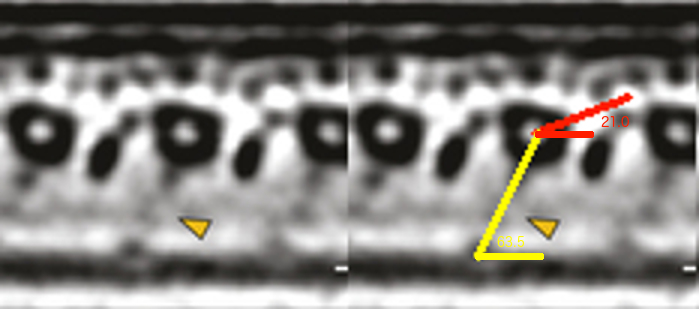
\includegraphics[width=.45\textwidth]{../figures/Post_powerstroke_tomography.jpg}
%%   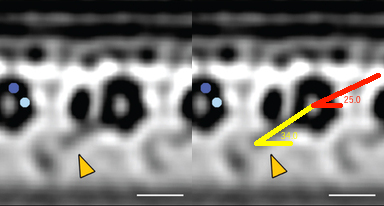
\includegraphics[width=.45\textwidth]{../figures/Pre_powerstroke_tomography.jpg}
%%   \caption{Post- and Pre-powerstroke equilibrium angles from EM tomography. Note: Ignore binding angle, the MTBD shouldn't actually be bound to MT.}
%%   \label{fig:em_tomography_eq_angles}
%% \end{figure}

\subsection{Linker position in Post-powerstroke dynein, two Post-PS states?}
Insights into dynein motor domain function from a 3.3A crystal structure, Hugo Schmidt, Andrew P. Carter\\

A crystal structure of just the motor domain in a low-ATP-affinity conformation. Suggests that differences between their structure and a Dictyostelium ADP-bound structure suggest there is a difference between AAA1 apo/ADP states, suggesting at least two post-powerstroke states. The paper postulates that linker interacting with AAA5 is what kicks out ADP. They say that linker-AAA5 complex creates a low-nucleotide-affinity state.\\

They further suggest that nucleotide binding causes the linker to unbind AAA5 and rebind AAA2 on nucleotide binding. Thus AAA5-linker is post-powerstroke apo and AAA2-linker is ATP-bound (pre or post powerstroke?)\\

ATPases 2, 3, 4 mutation leads to decreased velocity.\\

\subsection{Linker pre-powerstroke conformation}
ATP hydrolysis cycle-dependent tail motions in cytoplasmic dynein
Kon T, Sutoh K

This paper supposedly talks about how the linker changes conformation on ATP binding.\\

A FRET study on how ATP changes the distance of domains. They label the C-terminal tail and different regions on the motor, then calculate the FRET efficiency. FRETY efficiency is higher when ATP is present, indicating two different states based on ATP presence. They try to trap dynein in different states (apo, ATP, ADP-Pi, ADP) using different trapping nucleotide analogs. ADP-Vi dynein stayed in state II, while nonhydrolyzable ATP, apo, and ADP additions caused the motor to stay in state I.\\

The interpretation is that the dynein's tail moves from a state where it is near the C-terminus (AAA5) to one where it is near AAA2. 5->2 is prestroke on hydrolysis, 2->5 is poststroke on Pi rejection. ATP binding is what causes the conformation change, since they have trapped ATP-ish bound dyneins in both state I and II. The powerstroke happens during the ADP state, since they have an ADP-dynein in state II and another in state I.\\

They also report an ATPase $k_{cat} = 90.2 \pm 4.5$, meaning roughly 100 ATP are cycled per second.\\

\subsection{Possibly more equilibrium motor angles}
Dynein structure and power stroke
Nature 2003, Burgess and Oiwa

EM microscopy of apo/ADP-Vi flagellar dynein shows that the stem and stalk don't change length between two states, only the angle/position changes. The paper claims ``the origin of the movement is a displacement of the stem relative to the head and stalk.''.

Paper claims motor angle is \textbf{160 degrees in pre-stroke and 136 degrees in powerstroke}.\\

\textbf{Could we use the angle distribution histograms in \ref{fig:EM-angles-burgess} fit to a boltzmann factor with a spring energy to get cm?}

%% \begin{figure}[h!]
%%   \centering
%%   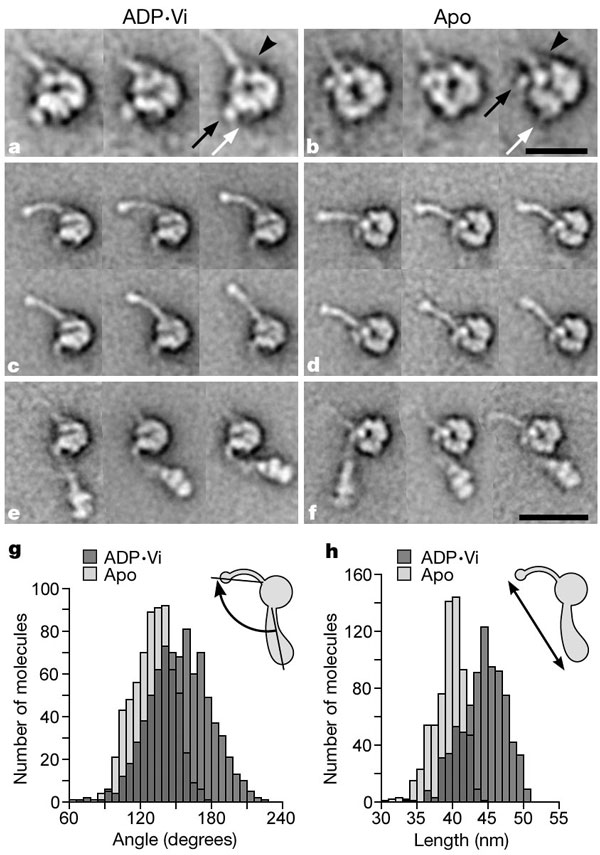
\includegraphics[width=.45\textwidth]{../figures/axonemal-motor-angles.jpg}
%%   \caption{Angle histograms from EM microscopy on axonemal (not cytoplasmic) dynein.}
%%   \label{fig:EM-angles-burgess}
%% \end{figure}


There is a difference in standard deviation of angles in pre/post-stroke. Pre-stroke has a stdev of 20 degrees, Post-stroke has a stdev of 11. The authors indicate this is due to stiffening of the stalk/foot domain. This seems like it would indicate changes in the motor spring constants between the pre/post-powerstroke states.

\subsection{2012 Kon Crystal Structure (3VKH)}
This paper crystallizes a full-length and MTBD-truncation mutants. 3VKH is the full-length, but one MTBD of the dimer did not come out in the crystal structure.

\subsection{Imamula Stepping Model}
This is an older (2007) paper presenting a chemical model and giving rate constants for MT un/binding. Averages are: $K_{d,pre} = 0.2uM$, $K_{d,post} > 10uM$. They determine these by adding a known concentration of monomeric Dynein apo, ATP, ADP-Pi or ADP, adding microtubules, removing MT-Dynein dimers and remeasuring concentration. These parameters are good in that equilibrium constants (as opposed to rate constants) \textit{don't} take into account kinetics, only free energy change...right?\\

Also, the paper says that axonemal dyneins have multiple motor domains, i.e aren't dimers, so that changes the results from the Lin paper. The binding angle is probably valid, though.\\

\subsection{Chemical Basis of Morphogenesis}
Turing paper on how asymmetry comes about in biology\\

\subsection{Coarge-grained modeling of the structural states and transition underlying the powerstroke of dynein motor domain}
Models six AAA+ domains, CC, C-term, pre/post-powerstroke\\

Modelling the motor domain, using the post-powerstroke crystal structure, and using ``normal mode analysis'' to create a fluid transition into the pre-powerstroke state. This involves taking a crystal structure and somehow calculating the number of normal mode angle changes necessary to get it from one state to another.\\

MD is hard on molecular motors, because their kinetic timescale is fairly slow.\\

Discusses Elastic Network Model - treating atoms as springs, then finding low-frequency normal modes of the whole protein\\

Choosing just a couple modes gets lots of information


\subsection{Further reading}
\begin{itemize}
\item The dynein family at a glance. Höök P, Vallee RB J Cell Sci. 2006 Nov 1; 119(Pt 21):4369-71. The actual differences between axonemal/cytoplasmic dynein.
\end{itemize}

\section{Notes by David}
(This stuff can be deleted or edited or moved elsewhere...)

The mean speed of dynein is $134\pm 60$~nm~s$^{-1}$.  It looks like
perhaps the speed should be more like 80 or 80 nm/s~\cite{reck2006single}.

Its average step 1D displacement is 8~nm. (See page 194 of Weihong's \emph{Nature} paper.)

Together this means that the mean time between steps is about 60~ms.
Note milliseconds.  Thus we really need to be careful about how small
our $\Delta t$ is.

Note also another paper that is very similar to that of Weihong~\cite{dewitt2012cytoplasmic}.

\section{Program Scaling}
Program runtimes, as of commit 62c4d:

\begin{verbatim}
elliotc12@bennet:~/dynein_walk$ grep "dt" default_parameters.h 
double dt = 1e-11;
elliotc12@bennet:~/dynein_walk$ time ./generate_stepping_data --runtime=1e-5
Running for 1e-05 s

real	0m5.001s
user	0m4.972s
sys	0m0.000s
elliotc12@bennet:~/dynein_walk$ time ./generate_stepping_data --runtime=1e-5
Running for 1e-05 s

real	0m7.121s
user	0m7.072s
sys	0m0.000s
elliotc12@bennet:~/dynein_walk$ time ./generate_stepping_data --runtime=1e-4
Running for 0.0001 s

real	0m26.666s
user	0m26.608s
sys	0m0.000s
elliotc12@bennet:~/dynein_walk$ time ./generate_stepping_data --runtime=1e-4
Running for 0.0001 s

real	0m29.479s
user	0m29.428s
sys	0m0.000s
elliotc12@bennet:~/dynein_walk$ time ./generate_stepping_data --runtime=1e-3
Running for 0.001 s

real	4m47.224s
user	4m46.832s
sys	0m0.000s
elliotc12@bennet:~/dynein_walk$ time ./generate_stepping_data --runtime=1e-3
Running for 0.001 s

real	4m56.207s
user	4m55.776s
sys	0m0.000s
elliotc12@bennet:~/dynein_walk$ time ./generate_stepping_data --runtime=1e-2
Running for 0.01 s

real	61m44.302s
user	61m35.264s
sys	0m0.120s
\end{verbatim}

The average time per iteration is ~3.9 microseconds, or 3.9e5 real seconds per simulated second at $dt=10^{-11}s$. Thus we can generate one 60-millisecond step in 23,400 seconds, or 6.5 hours. A thousand-step simulation would thus take, very roughly, 8 months.\\

\section{Todo}
\begin{itemize}
\item Add dt testing figure to thesis\_stuff.tex.
\item Make all figures in thesis\_stuff.tex be dependencies of thesis\_stuff.tex in the Makefile; it should be deducible to a novice how every figure is generated in code.
\item Check out kinetic parameters papers in the Winch model, see how they are aquired
\item Generate a figure explaining how our model simplifies the rate constants in the Winch paper / annual review.
\item Make a figure with PyMol visualizations with and without our model superimposed
\item Calculate Dynein motor efficiency by finding friction work on cargo and energy of ATP.
\item Make Dynein binding rate diagram showing how our model relates to the Imamula one
\item Make pretty dynein visualization in PyMol (or some software) showing how dimerization happens AND how docking to the MT happens; ask David what this should look like
\end{itemize}

\bibliographystyle{plain}
\bibliography{thesis_stuff}

\end{document}
